
\newpage

\begin{justify}
    Αν έχετε υλοποιήσει τα παραπάνω βήματα, 
    έχετε καταλάβει πως λειτουργεί ένα σύστημα 
    το οποίο χρησιμοποιεί διαμόρφωση \textlatin{16-QAM} 
    (φυσικά, έχουμε υποθέσει ότι το κανάλι είναι 
    ιδανικό και ότι είμαστε τέλεια συγχρονισμένοι).    
\end{justify}

\begin{justify}
    Στο δεύτερο μέρος, θα εκτιμήσετε την πιθανότητα 
    σφάλματος συμβόλου και \textlatin{bit} με χρήση της μεθόδου 
    \textlatin{Monte Carlo}.
\end{justify}

%------------------- Β.1 -------------------%

\begin{justify}
    {\bf 1.} Για $\textlatin{SNR}_{\textlatin{dB}} = [0 : 2 : 16]$, 
    να υπολογίσετε πειραματικά την πιθανότητα 
    σφάλματος απόφασης συμβόλου και bit επαναλαμβάνοντας 
    τα παραπάνω βήματα $K$ φορές (ενδεικτικά, $K = 200, 
    1000$) για κάθε \textlatin{SNR}.
\end{justify}

\begin{justify}
    {\bf Λύση:}\\
    Για τα διάφορα $\textlatin{SNR}_{\textlatin{dB}}$ και για $K=200$
    επαβαλήψεις, δημιουργήσαμε ακολουθίες από \textlatin{bit} και 
    ακολουθώντας τα βήματα του πρώτου μέρους, δημιουργήσαμε το 
    σήμα εξόδου. Ακολουθεί ο κώδικας για τον υπολογισμό
    της πειραματικής πιθανότητας σφάλματος απόφασης συμβόλου: 
\end{justify}

\vspace{-1cm}

%---------------------MATLAB code-----------------%

\textlatin{
    \lstinputlisting[language=Matlab,]{BETA/Matlab/b1.m}
}

%-------------------------------------------%

%------------------- Β.2 -------------------%

\begin{justify}
    {\bf 2.} Να σχεδιάσετε σε \textlatin{semilogy} τη
    θεωρητική και πειραματική πιθανότητα σφάλματος
    συμβόλου σαν συνάρτηση του $\textlatin{SNR}_{\textlatin{dB}}$.
    Τι παρατηρείτε\textlatin{;}
\end{justify}

\begin{justify}
    {\bf Λύση:}\\
    Χρησιμοποιώντας την συνάρτηση $Q$ όπως φαίνεται και από των παραπάνω
    κώδικα, σχεδιάσαμε σε κοινό \textlatin{semilogy} τη
    θεωρητική και πειραματική πιθανότητα σφάλματος
    συμβόλου.
\end{justify}

%-----------------------PLOT-b.2-------------------%

\begin{center}
    \centering
    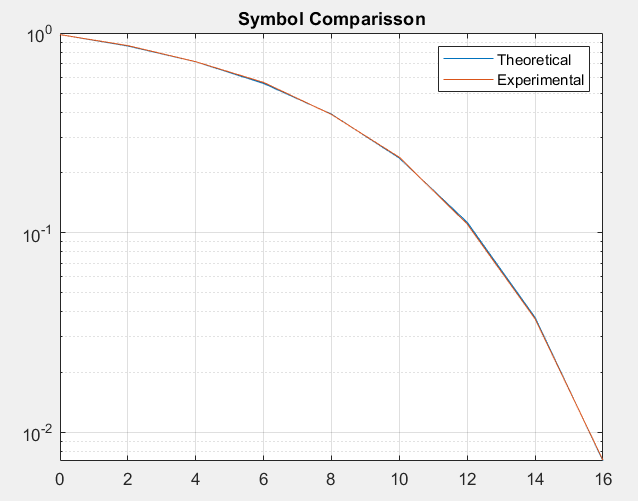
\includegraphics[width=0.8\textwidth]{BETA/IMAGES/b2.png} % Adjust width as neededfilename of your images
\end{center}

\begin{justify}
    Παρατηρείται ότι οι πειραματικές τιμές προσεγγίζουν τις θεωρητικές
    με πάρα πολύ καλή ακρίβεια.
\end{justify}

%-------------------------------------------%

%------------------- Β.3 -------------------%

\begin{justify}
    {\bf 3.} Να σχεδιάσετε σε \textlatin{semilogy} την
    πειραματική πιθανότητα σφάλματος \textlatin{bit} σαν
    συνάρτηση του $\textlatin{SNR}_{\textlatin{dB}}$.
    Στο ίδιο σχήμα, να σχεδιάσετε και τη θεωρητική
    προσέγγιση για την πιθανότητα σφάλματος \textlatin{bit}.
    Τι παρατηρείτε; Μπορείτε να εξηγήσετε το φαινόμενο\textlatin{;}
\end{justify}

\begin{justify}
    {\bf Λύση:}\\
    Όμοια με τα παραπάνω:
\end{justify}

%-----------------------PLOT-b.3-------------------%

\begin{center}
    \centering
    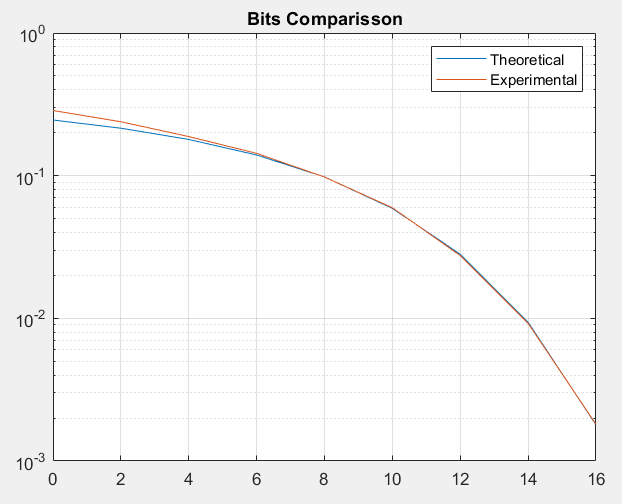
\includegraphics[width=0.8\textwidth]{BETA/IMAGES/b3.png} % Adjust width as neededfilename of your images
\end{center}

\begin{justify}
    Παρατηρούμε για μικρές τιμές του \textlatin{SNR}, το πειραματικό \textlatin{Rate}
    ξεπερνά το θεωρητικό όριο. Αυτό συμβάινει μιας και ο τύπος που χρησιμοποιήσαμε
    επαληθεύεται για μεγάλες τιμές \textlatin{SNR}.
\end{justify}


\begin{justify}
    Και ο κώδικας \textlatin{MatLab} για τα ερωτήματα {\bf 2} και 
    {\bf 3}:
\end{justify}

\vspace{-1cm}

%---------------------MATLAB code-----------------%

\textlatin{
    \lstinputlisting[language=Matlab,]{BETA/Matlab/b2-3.m}
}

%-------------------------------------------%

